\section{Aplicación de optimización matemática en Python}

En este capítulo se muestra el proceso de selección del algoritmo de optimizacion para la suite de simulación, con el cual será capaz de entregar los componentes físicos necesarios para el uso de una misión específica.

\subsection{Tipo de problema matemático}

Para seleccionar el tipo de optimizador adecuado, es fundamental entender el tipo de problema que abordará la suite de optimización. En este contexto, se define la función objetivo a minimizar de la siguiente manera:


\[
f(x) = \sum_{i=1}^{9} f_i \cdot P_i
\]
\[
\text{Sujeto a } x = \{ x \leq b_i, \ i=1, \dots, 9 \}
\]

Donde:
\[
x = (\sigma_s, \sigma_b, \tau)
\]
\[
f_i:  \text{Funciones de costo en base a rendimiento y costo.}
\]
\[
b_i: \text{Restricciones de componentes físicos.}
\]
\[
P_i: \text{Peso o relevancia asignada a cada $f_i$.}
\]

Además, $\sigma_s$ representa la desviación estándar del sensor solar, $\sigma_b$ la desviación estándar del magnetómetro, y $\tau$ el límite máximo de torque en los actuadores. Complementando esto, las funciones de costo se presentan en las Tablas~\ref{tab:f_rend} y \ref{tab:f_cost}. La primera tabla muestra las funciones basadas en los parámetros de rendimiento de apuntamiento (MoP), mientras que la segunda se enfoca en los costos de los componentes físicos, considerando la potencia promedio y la masa. 

En ambas tablas, la parte izquierda de la ecuación muestra el valor obtenido por la suite de simulación (MoP de apuntamiento) o la función representativa (SE envelopes de potencia y masa), mientras que la parte derecha indica el valor objetivo definido por el usuario. Para los parámetros de rendimiento, se consideran el promedio de las exactitudes de apuntamiento de los ángulos de Euler, la densidad espectral de potencia de la norma de los ángulos de Euler, y el mayor tiempo de asentamiento entre Roll, Pitch o Yaw, normalizado en función de la frecuencia natural del sistema espacio-estado. Este enfoque permite ajustar tanto los componentes físicos como los parámetros de apuntamiento de acuerdo con los requisitos específicos del usuario, garantizando que la optimización refleje las condiciones reales de la misión.

\begin{table}[H]
	\centering
	\caption{Funciones de costo en base a rendimiento.}
	\label{tab:f_rend}
	\begin{tabular}{|c|}
		\hline
		$f_1 = \left\lVert \text{Acc}(\sigma_m, \sigma_s, \tau) - \text{Acc} \right\rVert^2$ \\ \hline
		$f_2 = \left\lVert \text{Time}(\sigma_m, \sigma_s, \tau) - \text{Time} \right\rVert^2$ \\ \hline
		$f_3 = \left\lVert \text{Jitter}(\sigma_m, \sigma_s, \tau) - \text{Jitter} \right\rVert^2$ \\ \hline
	\end{tabular}
\end{table}

\begin{table}[H]
	\centering
	\caption{Funciones de costo en base a costo.}
	\label{tab:f_cost}
	\begin{tabular}{|c|}
		\hline
		$f_4 = \left[ \text{Masa}_{\text{mag}}(\sigma_m) - \text{Masa}_{\text{mag}} \right]^2$ \\ \hline
		$f_5 = \left[ \text{Pot}_{\text{mag}}(\sigma_m) - \text{Pot}_{\text{mag}} \right]^2$ \\ \hline
		$f_6 = \left[ \text{Masa}_{\text{sun}}(\sigma_s) - \text{Masa}_{\text{sun}} \right]^2$ \\ \hline
		$f_7 = \left[ \text{Pot}_{\text{sun}}(\sigma_s) - \text{Pot}_{\text{sun}}(i) \right]^2$ \\ \hline
		$f_8 = \left[ \text{Masa}_{\text{act}}(\tau) - \text{Masa}_{\text{act}} \right]^2$ \\ \hline
		$f_9 = \left[ \text{Pot}_{\text{act}}(\tau) - \text{Pot}_{\text{act}} \right]^2$ \\ \hline
	\end{tabular}
\end{table}

Es importante destacar que el usuario podrá seleccionar qué componentes físicos y MoP de apuntamiento optimizar, así como el tipo de actuador a simular en la suite de optimización. En cada caso, se excluirá la función $f_i$ correspondiente para adaptar la optimización a los requisitos específicos.

Independientemente del análisis, la función objetivo es de tipo General Nonlinear Programming (NLP), ya que las variables de optimización no presentan una relación lineal o cuadrática con la salida. Sin embargo, existen restricciones lineales que se basan en los límites mínimo y máximo de la masa y la potencia promedio de los componentes físicos. Finalmente, debido a la complejidad de la simulación de actitud, es necesario determinar si el problema es convexo o no, lo que influirá en la selección del solver o los optimizadores disponibles en Python que se pueden utilizar.

\subsection{Pruebas de convexidad en scipy.optimize}

Para determinar si el problema es convexo, se utiliza la librería scipy.optimize.minimize, especializada en la búsqueda de mínimos locales. Estos serían suficientes si la suite de simulación resultara ser convexa.

El análisis comienza con la presentación de las funciones representativas de la potencia y la masa de los componentes físicos. Para construir estas funciones, se recopilaron datos de componentes utilizados en CubeSats, generando un conjunto de puntos que permiten evaluar su comportamiento y obtener una curva representativa. Como ejemplo, en las Figuras \ref{fig:pot_mag} y \ref{fig:masa_magn} se muestran los pares ordenados de desviación estándar en relación con la potencia promedio y la masa de los magnetómetros, respectivamente. Las gráficas de los otros componentes se incluyen en el Anexo \ref{ap:Z9}.

\begin{figure*}[h!]
	\centering
	\begin{subfigure}[t]{0.6\textwidth}
		\centering{%
			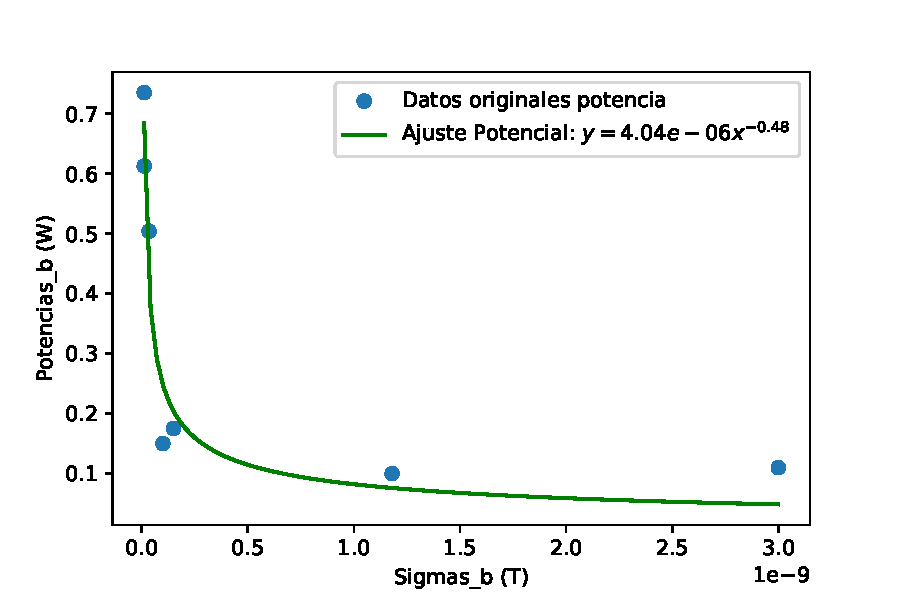
\includegraphics[width=\textwidth]{potencia_magn.pdf}
		}%
		\subcaption{Gráfica desviación estándar vs potencia prom de los magnetómetros.\label{fig:pot_mag}}
	\end{subfigure}
	\begin{subfigure}[t]{0.6\textwidth}
		\centering{%
			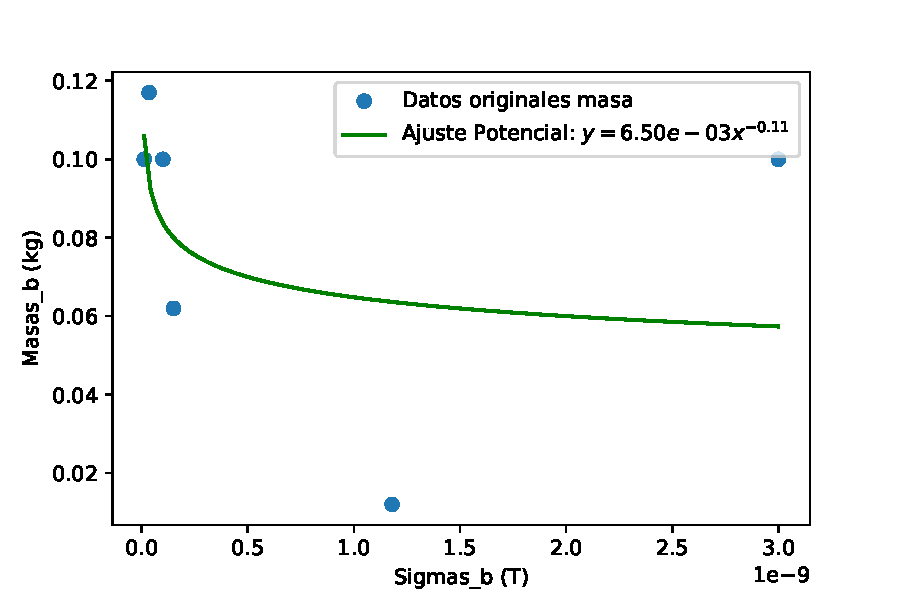
\includegraphics[width=\textwidth]{masa_magn.pdf}
		}%
		\subcaption{Gráfica desviación estándar vs masa de los magnetómetros.\label{fig:masa_magn}}
	\end{subfigure}
	\caption{Datos de masa y potencia promedio de magnetometros y su ajuste potencial.}\label{fig:magn_aj}
\end{figure*}

Con esta base, y sabiendo que las funciones de costo relacionadas con el rendimiento se derivan de la simulación del ADCS para los MoP de apuntamiento, se evaluaron dos casos específicos, considerando que como usuario se entrega MoP de apuntamiento y funciones de costo igual a 0. El primero consiste en optimizar únicamente el MoP de exactitud de apuntamiento (accuracy), utilizando solo sensores y magnetorquers como actuadores. El segundo caso analiza la optimización de todos los MoP de apuntamiento, considerando tanto sensores como actuadores del tipo magnetorquer.

En el primer caso, solo se incluyen en la función de costo global las funciones $f_1$, $f_4$, $f_5$, $f_6$, y $f_7$. En el segundo caso, se utilizan todas las funciones listadas en las Tablas \ref{tab:f_rend} y \ref{tab:f_cost}. Estos dos casos fueron seleccionados porque el primero representa un problema más sencillo, ya que solo optimiza un parámetro de rendimiento basado en los sensores. En contraste, el segundo caso es más complejo, al optimizar todos los MoP en función de los componentes del ADCS.

\subsubsection{Análisis caso de optimización simple.}

Para iniciar el análisis de convexidad, se configuró una malla de 20x20 puntos, evaluando 20 valores dentro de los límites inferiores y superiores de las desviaciones estándar del magnetómetro y del sensor solar, según los valores y parámetros del Capítulo 5. Esta grilla permite visualizar gráficamente la aproximación de la ubicación del mínimo global al considerar las funciones previamente descritas. La Figura \ref{fig:f_grilla3d} muestra esta grilla, donde los ejes x e y representan las desviaciones estándar evaluadas para el sensor solar y el magnetómetro, respectivamente, y el eje z corresponde al valor de la función de costo, acompañado por un mapa de colores que también representa esta función objetivo. A partir de estas evaluaciones, se logra minimizar la función a un valor de f(x) = 3.4928, obtenido en el par x = (0.641 [nT], 1.41[°]).

\begin{figure}[h!]
	\centering    
	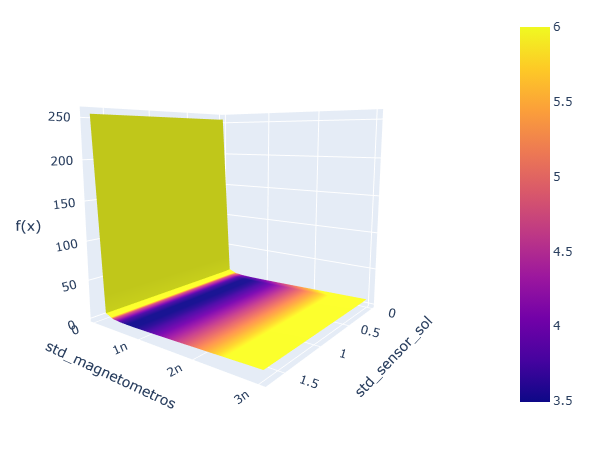
\includegraphics[width=0.8\textwidth]{SAboth0_typeact0_typerendacc.png}
	\caption{Grilla 20x20 caso número 1 de estudio de optimización.}
	\label{fig:f_grilla3d}
\end{figure}	

Con esta base, se realizó un análisis utilizando diferentes condiciones iniciales para la optimización con minimize, empleando diversos solvers. Se eligieron aquellos solvers que no requieren el cálculo del Hessiano, como L-BFGS-B, Nelder-Mead y Powell, debido a la dificultad de obtener la doble derivada de la suite de optimización en relación con las desviaciones estándar de los sensores.

Los resultados de la minimización para las condiciones iniciales de 1.5 [nT] y 0.5 [°] en los solvers mencionados se presentan en la Figura \ref{fig:acc_cond_inic_1}. Los valores obtenidos para la función objetivo son muy similares entre sí, incluso mostrando resultados inferiores al mínimo encontrado en la evaluación previa con la grilla.

Adicionalmente, se evaluaron diferentes condiciones iniciales para los sensores, utilizando 0.5 [nT] y 0.8 [°]. Los resultados obtenidos para los mismos solvers se muestran en la Figura \ref{fig:acc_cond_inic_2},  revelando valores prácticamente idénticos a los obtenidos con las primeras condiciones. El único solver que muestra ligeras diferencias es Nelder-Mead, aunque estas discrepancias son mínimas y pueden considerarse insignificantes.

\begin{figure}[h!]
	\centering
	\begin{subfigure}[b]{0.8\textwidth}
		\centering
		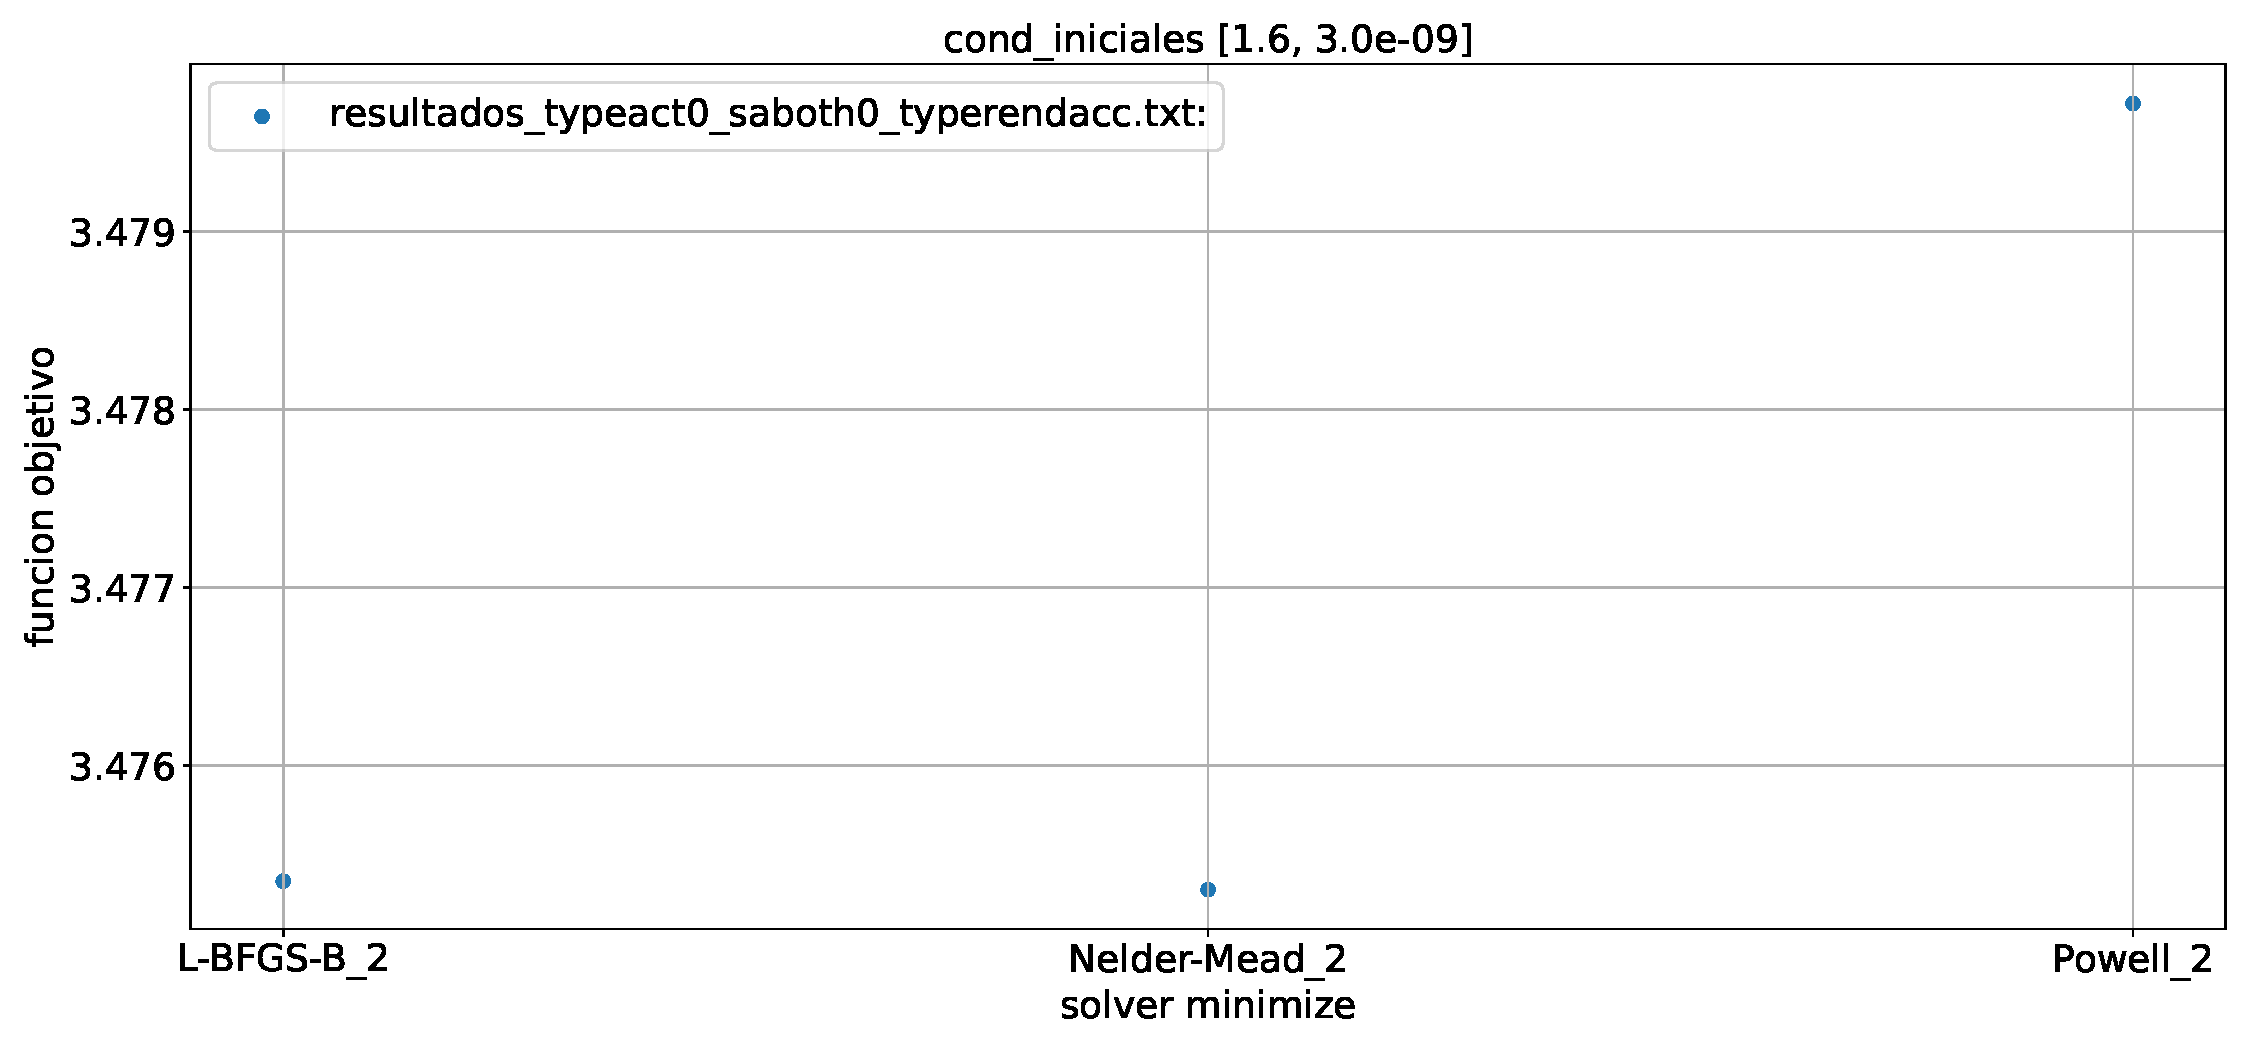
\includegraphics[width=\textwidth]{cond_iniciales_1.6_3.0e-9.pdf}
		\caption{Resultados con condiciones iniciales de 3.0 [nT] y 1.6 [°].}
		\label{fig:acc_cond_inic_1}
	\end{subfigure}
	\hfill
	\begin{subfigure}[b]{0.8\textwidth}
		\centering
		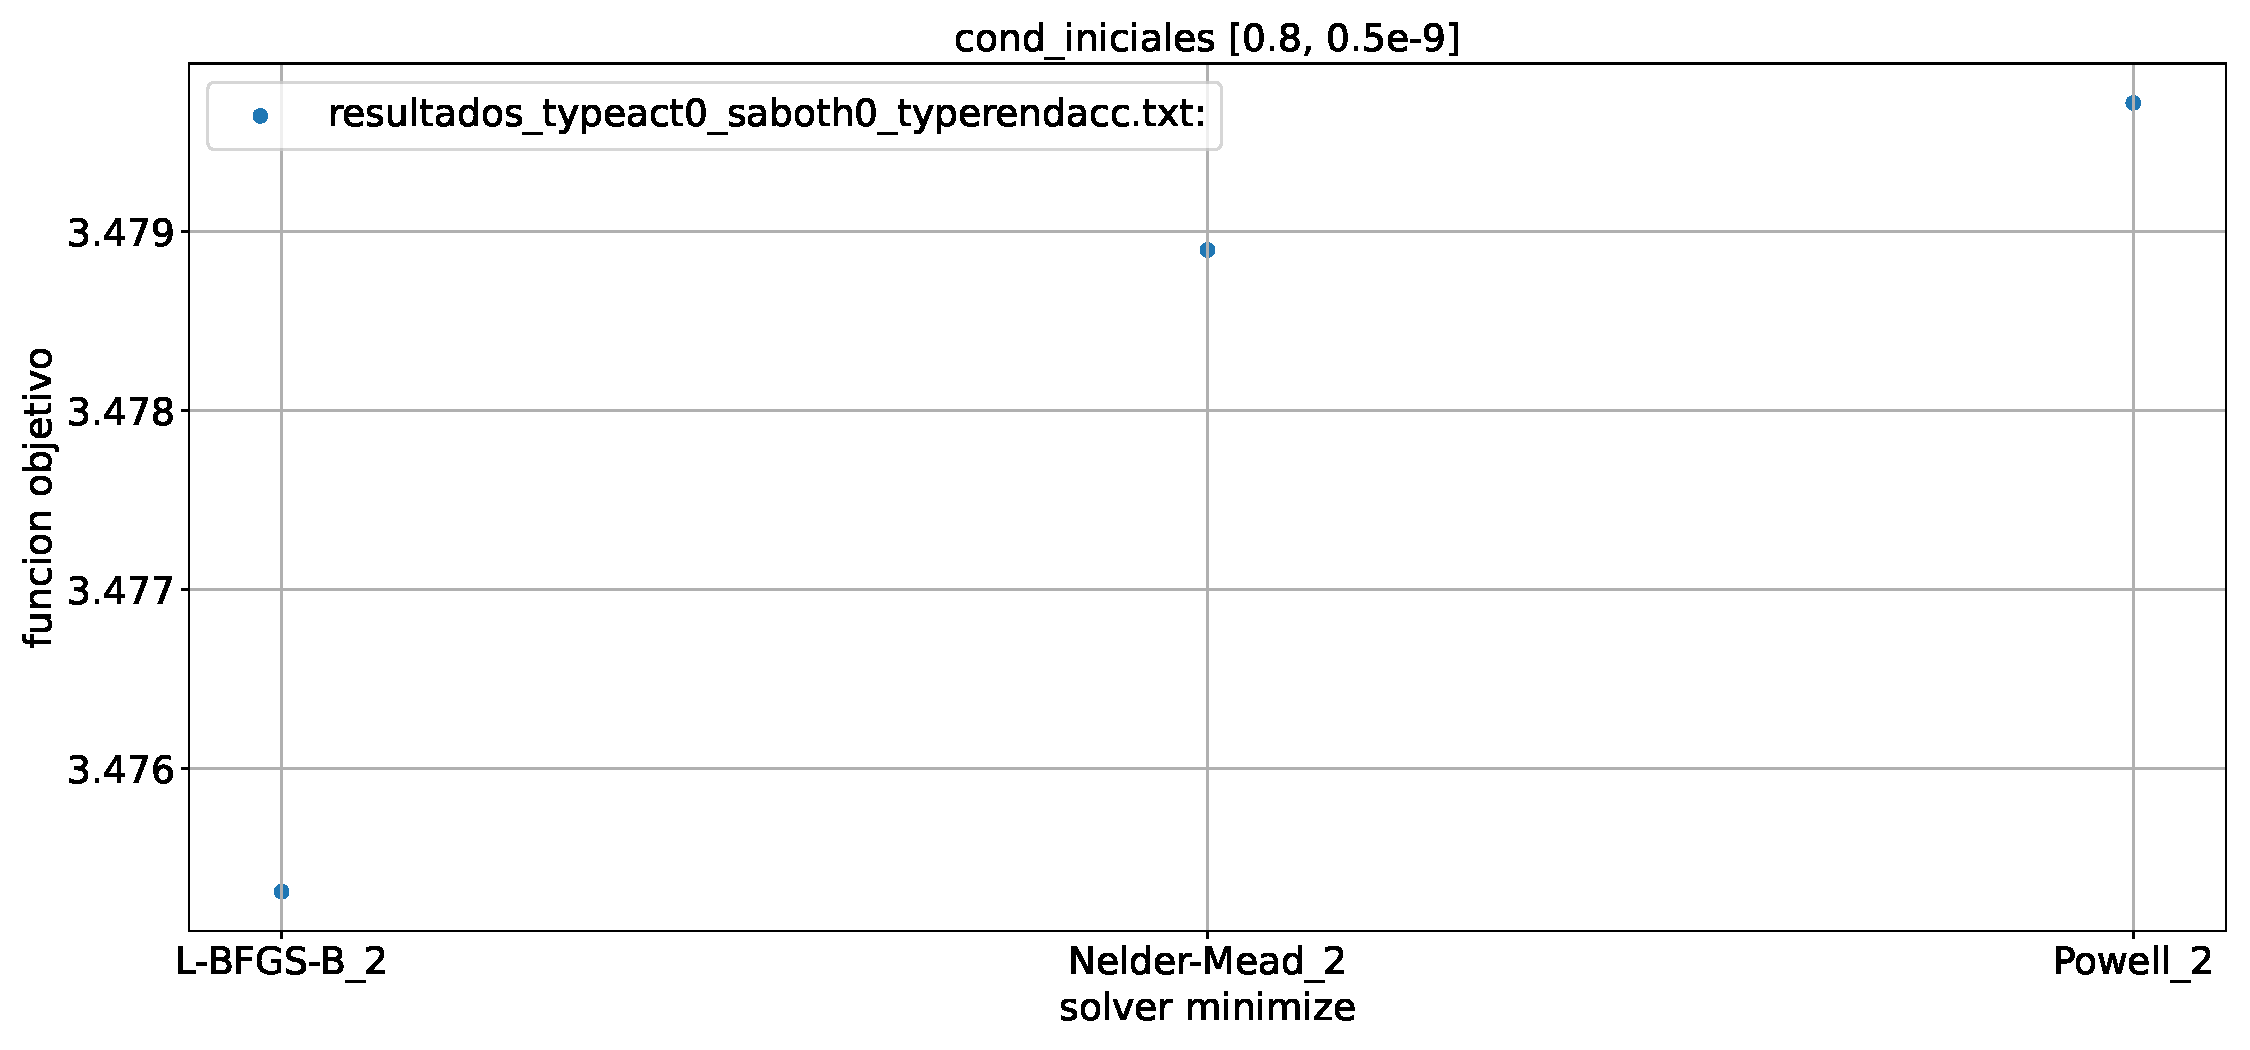
\includegraphics[width=\textwidth]{cond_iniciales_0.8_0.5e-9.pdf}
		\caption{Resultados con condiciones iniciales de 0.5 [nT] y 0.8 [°].}
		\label{fig:acc_cond_inic_2}
	\end{subfigure}
	\caption{Comparación de los resultados de la función objetivo simple con diferentes condiciones iniciales.}
	\label{fig:acc_cond_inic_comparacion}
\end{figure}

Por otro lado, se presentan condiciones iniciales que se encuentran en los extremos de las restricciones, las cuales se muestran en la Figura \ref{fig:acc_cond_inic_3} y \ref{fig:acc_cond_inic_4}. En todos los casos, se muestra ua variacion de al menos 3 milésimas en cada solver, al igual que los casos de estudio anteriores, siendo cualquier opción util en caso de querer optimizar solo un MoP de apuntamiento, con un componente físico.

\begin{figure}[h!]
	\centering
	\begin{subfigure}[b]{0.8\textwidth}
		\centering
		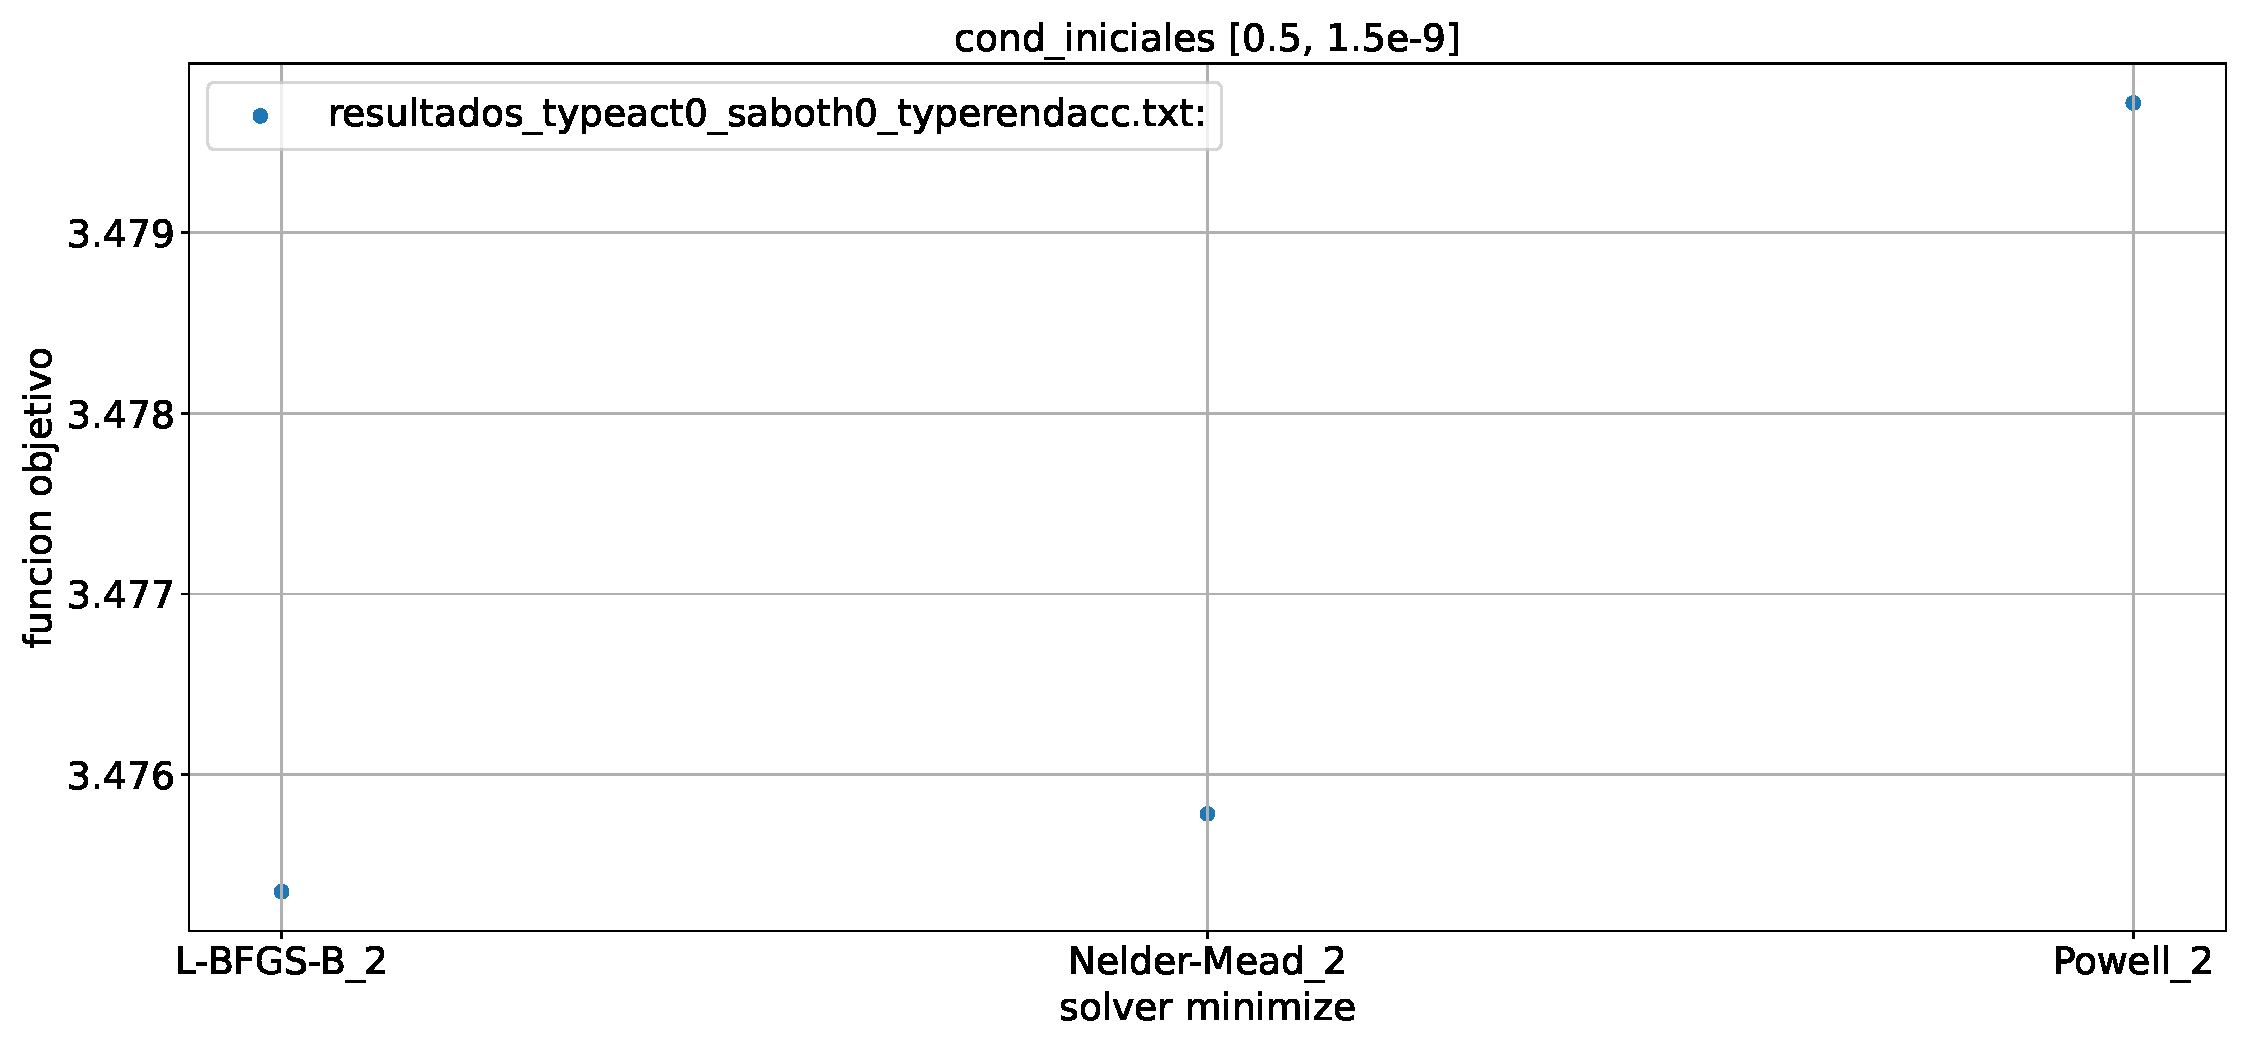
\includegraphics[width=\textwidth]{cond_iniciales_0.5_1.5e-9.pdf}
		\caption{Resultados con condiciones iniciales de 1.5 [nT] y 0.5 [°].}
		\label{fig:acc_cond_inic_3}
	\end{subfigure}
	\hfill
	\begin{subfigure}[b]{0.8\textwidth}
		\centering
		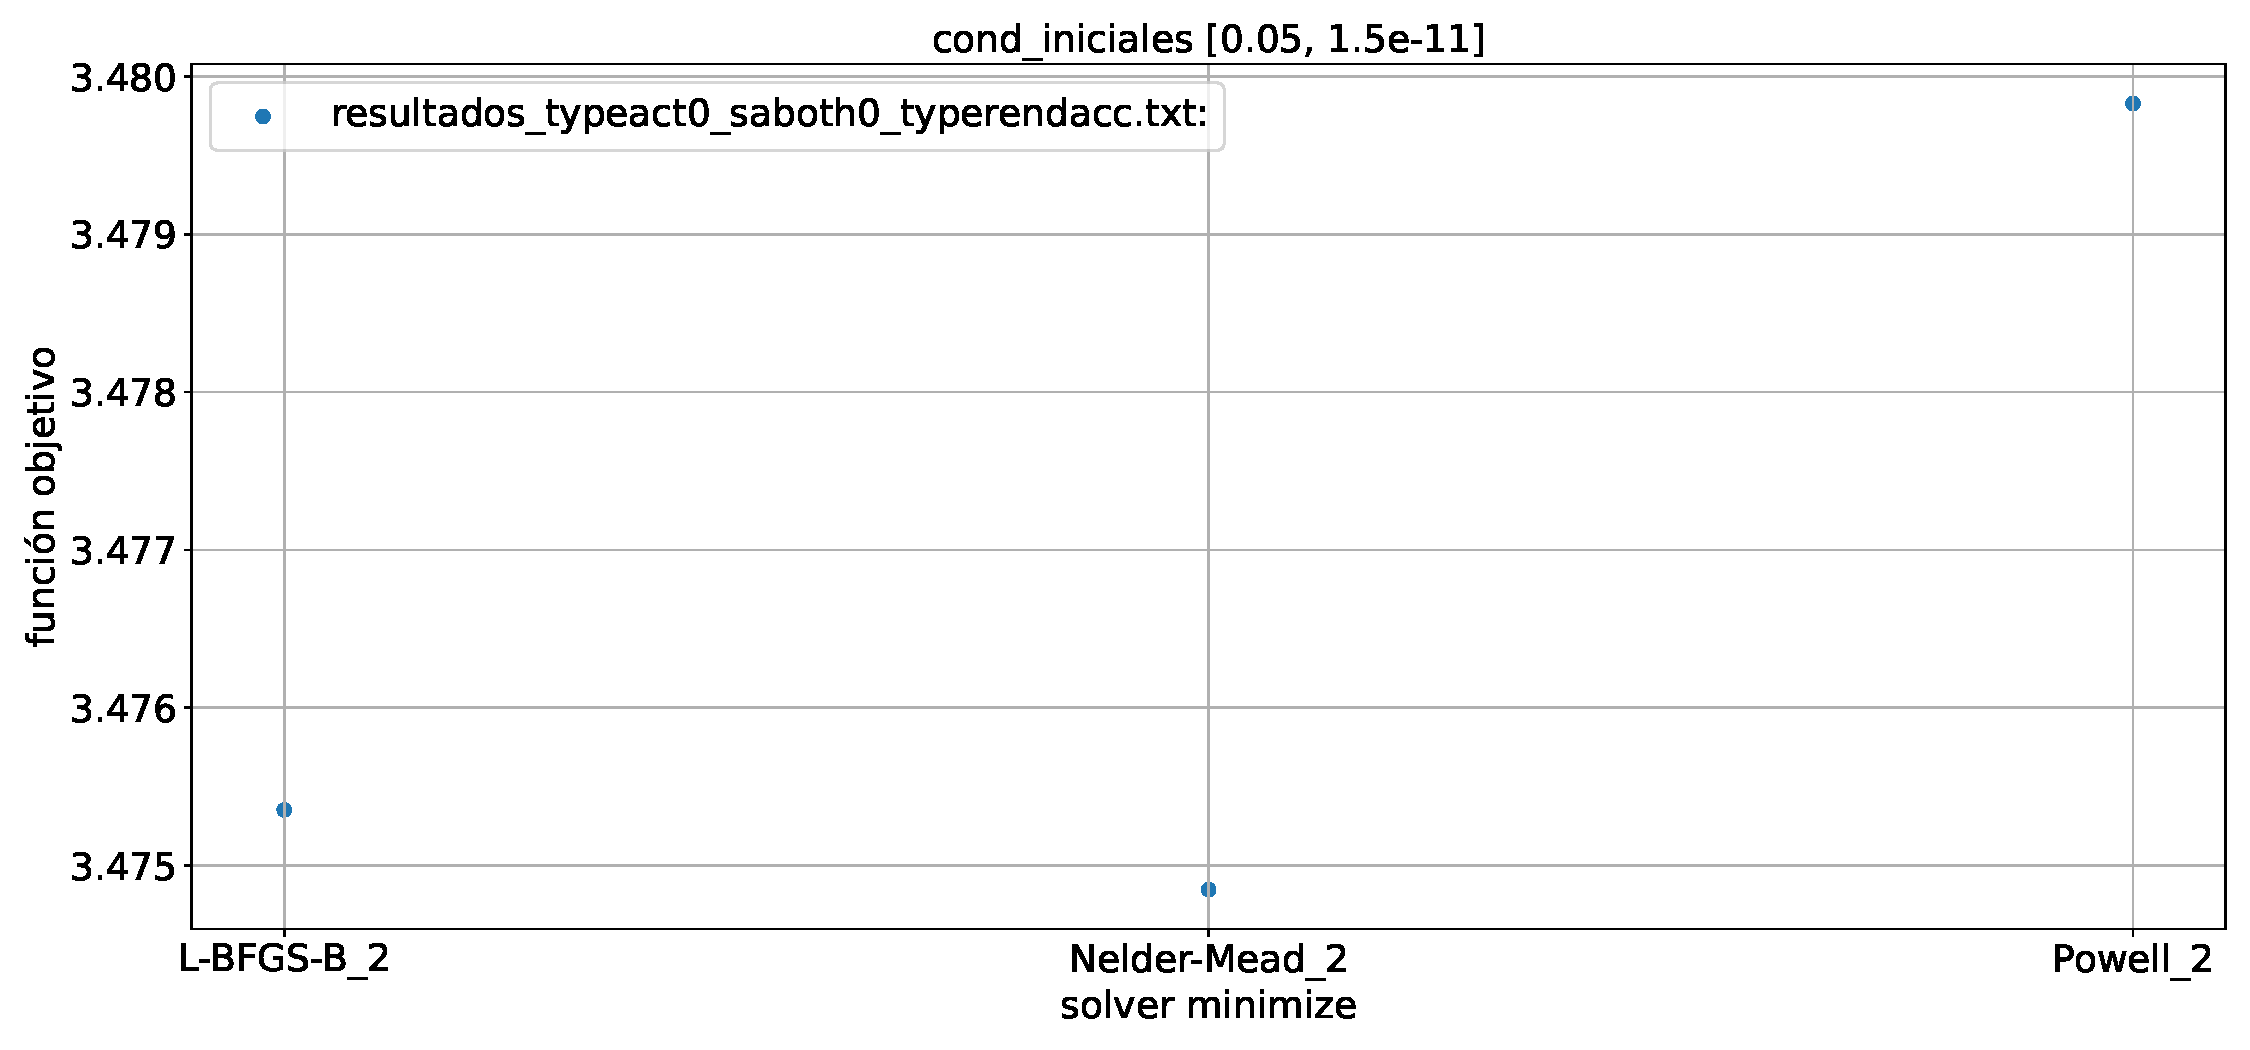
\includegraphics[width=\textwidth]{cond_iniciales_0.05_1.5e-11.pdf}
		\caption{Resultados con condiciones iniciales de 0.015 [nT] y 0.05 [°].}
		\label{fig:acc_cond_inic_4}
	\end{subfigure}
	\caption{Comparación de los resultados de la función objetivo simple con condiciones iniciales extremas.}
	\label{fig:acc_cond_inic_comparacion_ext}
\end{figure}

En base a estos caso, se puede observar que los solver de minimize son capaces de resolver este problema más sencillo otorgando una solución óptima.

\subsubsection{Análisis caso de optimización complejo.}

En este caso, se generó una malla de 20x20x6 puntos para evaluar las desviaciones estándar de los sensores y el límite de torque del magnetorquer dentro de un rango determinado, similar al análisis previo. En esta grilla, los ejes x, y y z representan las variables de optimización, mientras que el mapa de colores refleja la variación en los resultados de la función objetivo, permitiendo identificar la posible ubicación de un mínimo global. La grilla se presenta en la Figura \ref{fig:f_grilla4d}, donde se obtiene un valor mínimo global de 4.2171, alcanzado en los valores óptimos de 2.21 [nT], 0.36 [°] y 14.23 [A$m^{2}$].

\begin{figure}[h]
	\centering    
	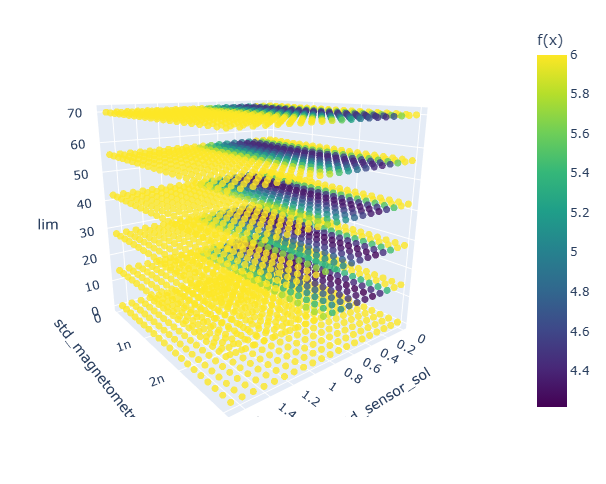
\includegraphics[width=0.8\textwidth]{SAboth2_typeact0_typerendall.png}
	\caption{Grilla 20x20x6 caso número 2 de estudio de optimización.}
	\label{fig:f_grilla4d}
\end{figure}	

Al igual que en el caso de optimización simple, aquí se probaron cuatro condiciones iniciales para evaluar si los solvers son capaces de aproximarse al valor mínimo global obtenido en la grilla.

Los resultados para los primeros casos de condiciones iniciales se presentan en las Figuras \ref{fig:all_cond_inic_1} y \ref{fig:all_cond_inic_2}. En la primera figura, se observa que los solvers L-BFGS-B y Powell logran valores cercanos al mínimo global, mientras que Nelder-Mead muestra una diferencia de 0.6 respecto al objetivo. En el segundo caso, Nelder-Mead alcanza el mismo mínimo que en el primer intento, mientras que L-BFGS-B se queda atrapado en otro mínimo local, distante del objetivo deseado. Por otro lado, Powell logra nuevamente alcanzar el mínimo esperado, lo que lo posiciona como un solver más confiable para este tipo de problema.

\begin{figure}[h!]
	\centering
	\begin{subfigure}[b]{0.8\textwidth}
		\centering
		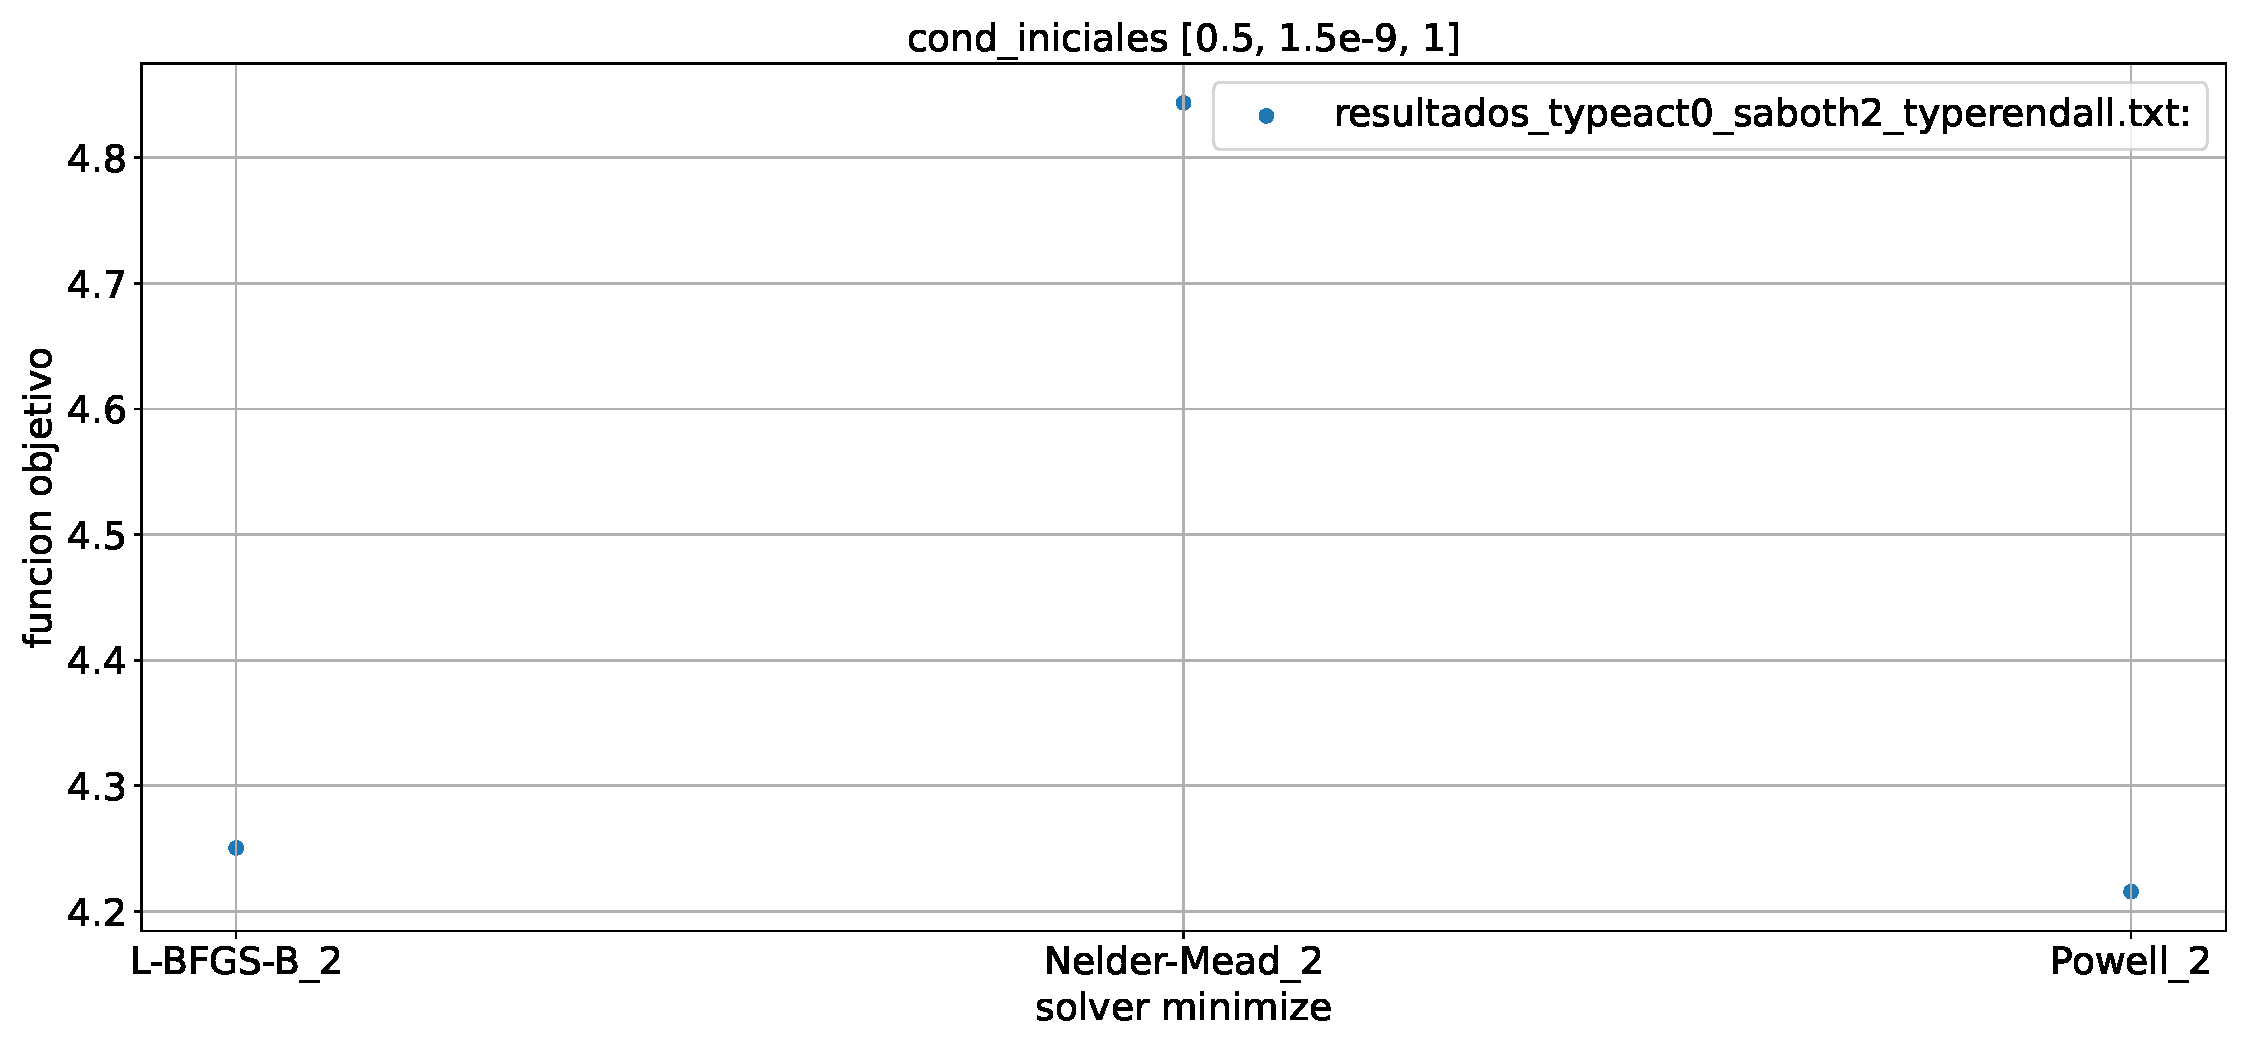
\includegraphics[width=\textwidth]{cond_iniciales_0.5_1.5e-9_1.0.pdf}
		\caption{Resultados con condiciones iniciales de 1.5 [nT], 0.5 [°] y 1.0 [A$m^2$].}
		\label{fig:all_cond_inic_1}
	\end{subfigure}
	\hfill
	\begin{subfigure}[b]{0.8\textwidth}
		\centering
		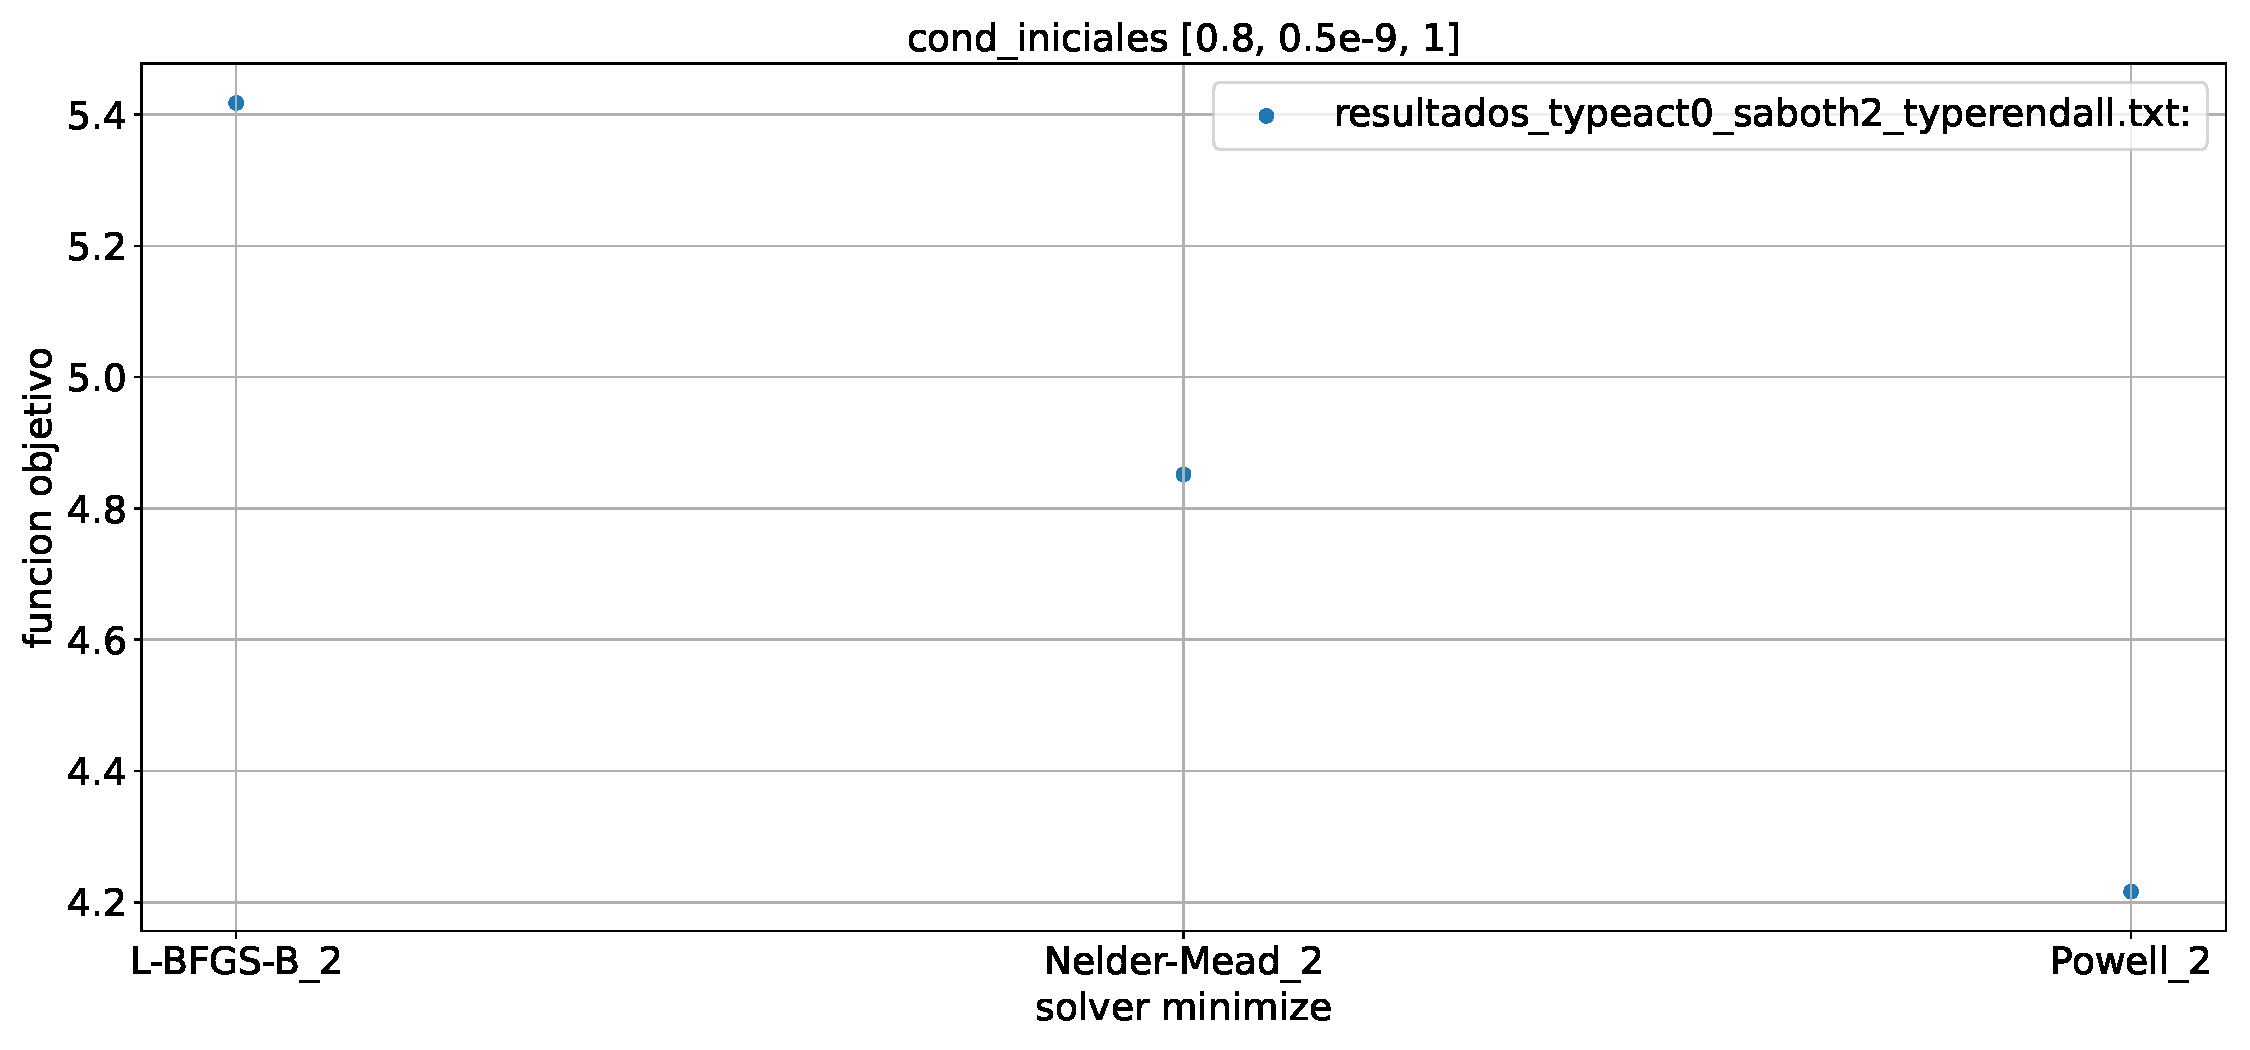
\includegraphics[width=\textwidth]{cond_iniciales_0.8_0.5e-9_1.0.pdf}
		\caption{Resultados con condiciones iniciales de 0.5 [nT], 0.8 [°] y 1.0 [A$m^2$].}
		\label{fig:all_cond_inic_2}
	\end{subfigure}
	\caption{Comparación de los resultados de la función objetivo compleja con diferentes condiciones iniciales.}
	\label{fig:cond_iniciales_comparacion}
\end{figure}

Además, se probaron dos casos adicionales con condiciones iniciales extremas, es decir, cercanas a los límites inferiores y superiores de las restricciones de las variables de optimización. Los resultados se presentan en las Figuras \ref{fig:all_cond_inic_3} y \ref{fig:all_cond_inic_4}. En el primer caso extremo, tanto L-BFGS-B como Nelder-Mead quedaron atrapados nuevamente en mínimos locales, más alejados del objetivo deseado, con valores de 11 y 6.2, respectivamente. Sin embargo, Powell logró alcanzar nuevamente el valor mínimo esperado. Para el segundo caso extremo, Nelder-Mead, al igual que Powell, logró llegar al mínimo global identificado en la grilla. Estos resultados refuerzan la fiabilidad de Powell para este tipo de problema, incluso en condiciones iniciales más extremas.


\begin{figure}[h!]
	\centering
	\begin{subfigure}[b]{0.8\textwidth}
		\centering
		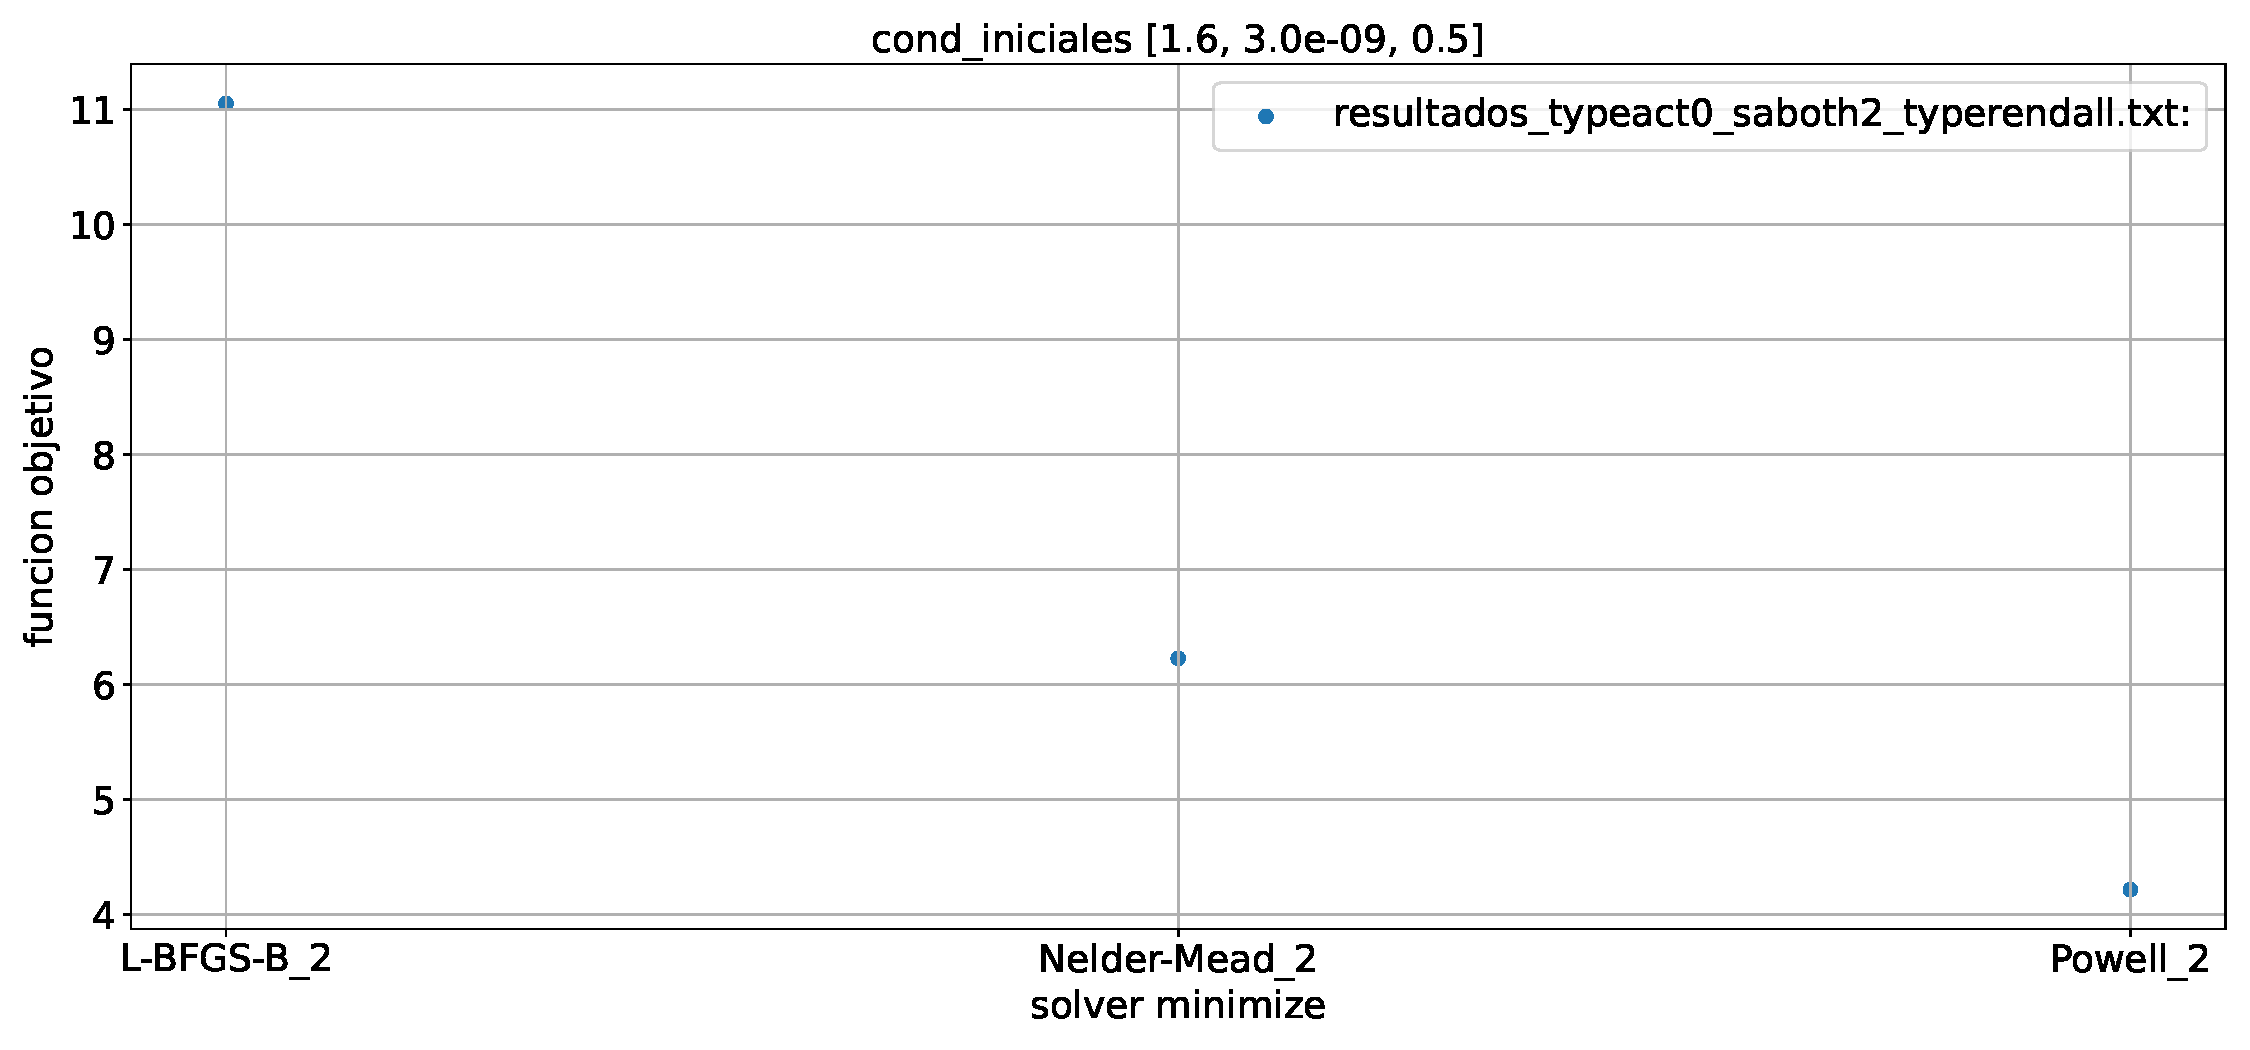
\includegraphics[width=\textwidth]{cond_iniciales_1.6_3.0e-9_0.5.pdf}
		\caption{Resultados con condiciones iniciales de 3 [nT], 1.6 [°] y 0.5 [A$m^2$].}
		\label{fig:all_cond_inic_3}
	\end{subfigure}
	\hfill
	\begin{subfigure}[b]{0.8\textwidth}
		\centering
		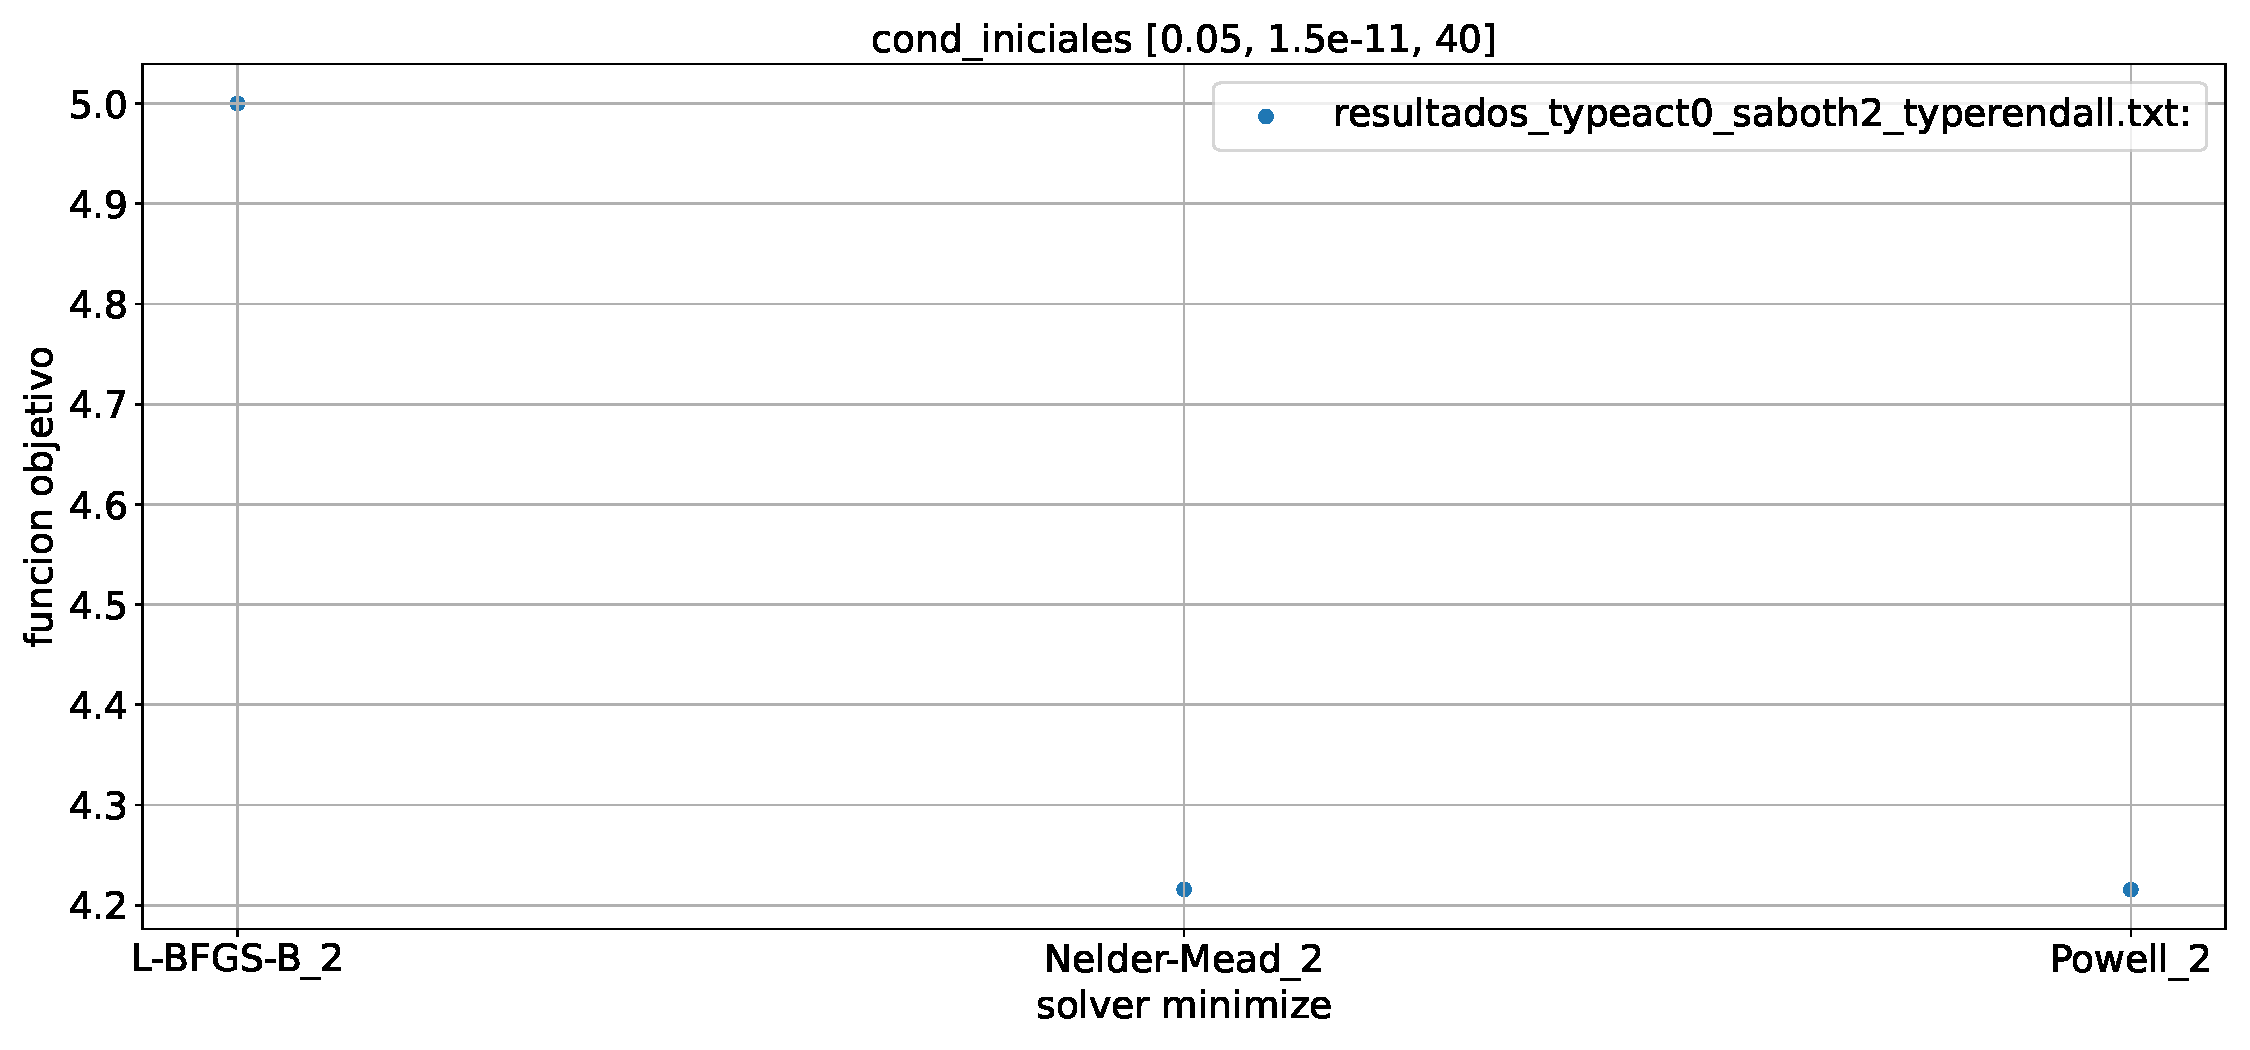
\includegraphics[width=\textwidth]{cond_iniciales_0.05_1.5e-11_40.pdf}
		\caption{Resultados con condiciones iniciales de 0.015 [nT], 0.05 [°] y 40 [A$m^2$].}
		\label{fig:all_cond_inic_4}
	\end{subfigure}
	\caption{Comparación de los resultados de la función objetivo compleja con condiciones iniciales extremas.}
	\label{fig:cond_iniciales_comparacion_2}
\end{figure}

\subsubsection{Análisis de Convexidad y Elección del Método de Optimización}

A partir de los análisis realizados en los apartados anteriores, es posible evaluar la convexidad del problema de optimización en base a los resultados obtenidos con distintos solvers y bajo diferentes condiciones iniciales. Se realizaron experimentos tanto con condiciones iniciales intermedias como extremas, utilizando los solvers L-BFGS-B, Nelder-Mead, y Powell, todos ellos apropiados para problemas donde no se cuenta con el Hessiano explícito.

En primer lugar, las pruebas realizadas con condiciones iniciales estándar para los dos casos de estudio—el simple (optimización de un solo MoP de apuntamiento) y el completo (optimización de todos los MoP)—indicaron que los resultados varían entre los solvers. En el caso más sencillo, tanto L-BFGS-B como Powell y Nelder-Mead lograron acercarse al valor mínimo global obtenido mediante la grilla de puntos. En el caso de optimización completa, los resultados fueron similares, aunque L-BFGS-B se quedó atrapado en un mínimo local en algunas ocasiones, mientras que Powell demostró una mayor consistencia, alcanzando el mínimo global en todos los intentos.

Por otro lado, al probar con condiciones iniciales extremas, tanto L-BFGS-B como Nelder-Mead se vieron atrapados nuevamente en mínimos locales más alejados del valor global. Sin embargo, Powell destacó al encontrar el mínimo global en todas las situaciones, mostrando su capacidad para evitar mínimos locales y converger hacia el mínimo deseado, incluso en escenarios más complicados.

Estos resultados sugieren que el problema no es convexo. Si fuera convexa, todos los solvers habrían convergido de manera consistente hacia el mismo valor óptimo, independientemente de las condiciones iniciales. La presencia de múltiples mínimos locales y el hecho de que algunos solvers quedaran atrapados en ellos refuerza la idea de que el problema tiene una naturaleza no convexa. La complejidad de la superficie de la función objetivo, combinada con restricciones lineales y la dependencia no lineal entre las variables de optimización y la salida, confirma que el problema es de tipo General Nonlinear Problem (GNP), lo que justifica la variabilidad en los resultados según el método de optimización empleado.

Finalmente, dada la performance de los solvers, Powell surge como una alternativa prudente y robusta para la resolución de este tipo de problemas. Su capacidad para evitar mínimos locales y alcanzar consistentemente el valor mínimo global lo convierte en la opción más confiable entre los solvers probados, especialmente en problemas con características no convexas como el presente.